
\documentclass{template/openetcs_article}
% Use the option "nocc" if the document is not licensed under Creative Commons
%\documentclass[nocc]{template/openetcs_article} 
\usepackage[pdftex]{hyperref}
\usepackage{lipsum,url}
\usepackage{xspace}
\usepackage{graphicx}
\usepackage{fixme}
\usepackage{lscape} 
\usepackage{pgfgantt}
\usepackage{adjustbox}
\usepackage{datetime}
\usepackage{listings}
\usepackage{placeins}
\usepackage{framed}
\usepackage{booktabs}

\numberwithin{figure}{section}
\numberwithin{table}{section}
\usepackage{float}
\floatstyle{plain}
\newfloat{listing}{thp}{lop1}[section]
\floatname{listing}{Listing}


\def\CC{{C\nolinebreak[4]\hspace{-.05em}\raisebox{.4ex}{\tiny\bf ++}}}


%user specified macros


\newcommand{\VV}{Verification \& Validation\xspace}
\newcommand{\vv}{verification \& validation\xspace}

\def\CC{{C\nolinebreak[4]\hspace{-.05em}\raisebox{.4ex}{\tiny\bf ++}}}

\newcommand{\bitwalker}{\mbox{\texttt{Bitwalker}}\xspace}

\newcommand{\poke}{\mbox{\texttt{Bitwalker\_Poke}}\xspace}
\newcommand{\peek}{\mbox{\texttt{Bitwalker\_Peek}}\xspace}
\newcommand{\acsl}{\mbox{\textsf{ACSL}}\xspace}
\newcommand{\isoc}{\mbox{\textsf{C}}\xspace}
\newcommand{\framac}{\mbox{\textsf{Frama-C}}\xspace}
\newcommand{\framacwp}{\mbox{\textsf{Frama-C\slash WP}}\xspace}
\newcommand{\why}{\mbox{\textsf{Why}}\xspace}
\newcommand{\wpframac}{\mbox{\textsf{WP}}\xspace}
\newcommand{\altergo}{\mbox{\textsf{Alt-Ergo}}\xspace}
\newcommand{\qed}{\mbox{\textsf{Qed}}\xspace}
\newcommand{\cvc}{\mbox{\textsf{CVC4}}\xspace}
\newcommand{\z}{\mbox{\textsf{Z3}}\xspace}
\newcommand{\coq}{\mbox{\textsf{Coq}}\xspace}
\newcommand{\cealist}{\mbox{\textsf{CEA LIST}}\xspace}

\newcommand{\inl}[1]{\lstinline[style=inline]{#1}}


%Defining C-Code Environment

\usepackage{courier} 
\usepackage{listings}
\usepackage{color} 

% fix bug with listing under texlive-2014
% see https://lists.debian.org/debian-tex-maint/2014/06/msg00209.html

\makeatletter
\renewcommand\lstinline[1][]{%
  \leavevmode\bgroup % \hbox\bgroup --> \bgroup
  \def\lst@boxpos{b}%
  \lsthk@PreSet\lstset{flexiblecolumns,#1}%
  \lsthk@TextStyle
  \ifnum\iffalse{\fi`}=\z@\fi
  \@ifnextchar\bgroup{%
  \ifnum`{=\z@}\fi%
  \afterassignment\lst@InlineG \let\@let@token}{%
  \ifnum`{=\z@}\fi\lstinline@}}
\makeatother


%\definecolor{darkred}		{rgb}{0.60,0.00,0.00}
\definecolor{coACSLBehavior}	{rgb}{0.30,0.00,0.00}
\definecolor{coASCL}		{rgb}{0.00,0.10,0.00}
\definecolor{coASCLKeyword}	{rgb}{0.00,0.10,0.10}
\definecolor{darkgreen}		{rgb}{0.00,0.40,0.00}
%\definecolor{red}		{rgb}{0.98,0.00,0.00}
\definecolor{darkblue}		{rgb}{0.00,0.00,0.60}
%\definecolor{lightblue}		{rgb}{0.60,0.80,1.00}
%\definecolor{lightred}		{rgb}{1.00,0.60,0.60}
\definecolor{coCKeyword}	{rgb}{0.00,0.00,0.60}

\lstdefinestyle{acsl-block}
{	emph=[1]{assert, assumes, assigns, axiom, axiomatic, decreases, ensures,
                 ghost, invariant, lemma, logic, loop, predicate,
		 reads, requires, variant},
	emphstyle=[1]{\bfseries\color{coASCLKeyword}},
	emph=[2]{behavior, behaviors, complete, disjoint, for:},
	emphstyle=[2]{\bfseries\color{coACSLBehavior}},
	emph=[3]{typedef, int, char, integer, real, bool, size_type, value_type, uint8_t,  uint64_t},
	emphstyle=[3]{\bfseries\color{coCKeyword}},
	escapeinside={//`}{`//},
	morecomment=*[l][\color{coASCL}]{//@},
	morecomment=*[s][\color{coASCL}]{/*@}{*/},
	moredelim=*[is][\bfseries]{|*}{*|},
	%emphstyle=[3]{\ttfamily}
	}

\lstdefinestyle{func-decl}
{	emph=[1]{assert, assumes, assigns, axiom, axiomatic, decreases, ensures,
                 ghost, invariant, lemma, logic, loop, predicate,
		 reads, requires, variant},
	emphstyle=[1]{\bfseries\color{coASCLKeyword}},
	emph=[2]{behavior, behaviors, complete, disjoint, for:},
	emphstyle=[2]{\bfseries\color{coACSLBehavior}},
	emph=[3]{integer, real, size_type, value_type},
	emphstyle=[3]{\bfseries\color{coCKeyword}},
	escapeinside={//`}{`//},
	morecomment=*[l][\color{coASCL}]{//@},
	morecomment=*[s][\color{coASCL}]{/*@}{*/},
	moredelim=*[is][\bfseries]{|*}{*|},
    frame=none,
    numbers=none
	%emphstyle=[3]{\ttfamily}
	}

\lstdefinestyle{acsl-inline}
{	emph=[1]{assert,assigns, assumes, axiom, axiomatic, decreases, ensures, ghost, invariant, lemma, logic, loop,
             predicate, reads, requires, return, variant },
	emphstyle=[1]{\bfseries\color{coASCLKeyword}},
	emph=[2]{behavior, behaviors, complete, disjoint, for:},
	emphstyle=[2]{\bfseries\color{coACSLBehavior}},
	emph=[3]{typedef, int, char, integer, real, bool, size_type, value_type, uint8_t,  uint64_t},
	emphstyle=[3]{\bfseries\color{coCKeyword}},
	morecomment=*[l][\color{coASCL}]{//@},
	morecomment=*[s][\color{coASCL}]{/*@}{*/},
	moredelim=*[is][\bfseries]{|*}{*|}
}

\lstdefinestyle{inline}
{      % basicstyle = \ttfamily\small\color{coASCL},
	keywordstyle = \ttfamily\small\color{coASCL},
	stringstyle=\color{coASCL},
	style=acsl-inline,
	breaklines= false
}

\lstset{%
  language=C++,
  defaultdialect=ansi,
  basicstyle=\small\ttfamily,
  commentstyle=\small\color{darkgreen},
  keywordstyle=\small\bfseries\color{darkblue},
  stringstyle=\small\color{darkgreen},
  tabsize = 2,
  showspaces=false,
  showtabs=false,
  columns=fixed,  
  frame=none,  
  breaklines=true,
  showstringspaces=false,
  xleftmargin=0.2cm,
  %rangeprefix=//label, % to specify a certain range from a file
  %rangesuffix=;, % to be shown
  %includerangemarker=false,
	numbers=none
}


\graphicspath{{./template/}{.}{./images/}}
\begin{document}
\frontmatter
\project{openETCS}

%Please do not change anything above this line
%============================
% The document metadata is defined below

%assign a report number here
\reportnum{OETCS/WP4/D4.2.2}

%define your workpackage here
\wp{Work Package 4: ``Validation \& Verification Strategy''}

%set a title here
\title{First Validation and Verification Report on Implementation/Code}

%set a subtitle here
%\subtitle{Description of Work}

%set the date of the report here
\date{December 2013}

%define a list of authors and their affiliation here

\author{Marc Behrens}

\affiliation{DLR, WP4 Leader}
 
\author{Jens Gerlach, Kim Völlinger, Andreas Carben}

\affiliation{Fraunhofer FOKUS, WP4.3 Task Leader (Validation and Verification of Implementation/Code)}

\author{Izaskun de la Torre}
\affiliation{Software Quality Systems S.A.}

% define the coverart
\coverart[width=350pt]{openETCS_EUPL}

%define the type of report
\reporttype{Description of work}


\begin{abstract}
  This work package will comprise the activities concerned with
  verification and validation within openETCS. This includes \vv of
  development artifacts, that is, showing that models and code
  produced correctly express or implement what they are supposed
  to. And also, methods and tools to perform such tasks will be
  evaluated with the goal of assembling a suitable method and tool
  chain to support a full development.
\end{abstract}

%=============================
%Do not change the next three lines
\maketitle
\tableofcontents
\listoffiguresandtables
\newpage
%=============================

% The actual document starts below this line
%=============================


%Start here

%-----------------------------------------------------------------------
\section*{Introduction}
%-----------------------------------------------------------------------

\subsection*{Objectives}

\emph{Verification} is the activity to ascertain that a particular
step in the development has achieved its goals, i.e., that its result
correctly refines or implements its input, which may be a higher-level
design or a specification. \emph{Validation} is about making sure that
the end result of the development meets its initial specification,
that is, the requirements of the user. The term validation is also
used when a design artifact is checked against requirements from
previous steps. Verification and/or validation is required for most
development artifacts.  What exactly has to be checked depends on the
set of items produced in the development process, their role and their
nature.  As the EVC software contributes to several safety-critical
functions of the ETCS onboard unit, the specific requirements
concerning the safety aspects of the standards EN~50128 and EN~50129
have to be respected throughout.

A main obligation of this work package is the verification or
validation of development artifacts produced by WP~3. This work will
concentrate on the functional and safety aspect. Besides \vv,
the work package shall also establish a coherent and comprehensive
chain of methods and tools for V\&V in cooperation with WP~7. Specific
challenges in this respect arise from the wish to use models
extensively in the development process, which means that more common
approaches have to be improved or substituted to fit a
model-based development style, and from the requirement of
using open-source tools, or even trying to realize the EVC software as
an \emph{open proof} item.

In pursuing these goals, the work package generates feedback
concerning the adequacy, correctness and safety of development
artifacts for WP~3, and the usefulness of tools and methods for WP~7.  

\subsection*{Organisation of the Work package}

The work packages consists of five tasks. The first task defines the
\vv strategy and formulates the initial \vv plan. This plan defines the
\vv activities to be done in openETCS and proposes the means to
perform them. In later stages of the project the plan will be extended
and revised to reflect the findings made while applying methods and
tools to the artifacts at hand.

Both model and code of the EVC software are subjected to \vv as they
are produced by WP~3, and the tools and methods proposed in the \vv
plan as well as newly developed or improved tools from WP~7 are applied
and evaluated in the process. Findings from these steps are
iteratively fed back to the respective work package and used to refine
the \vv plan.

A dedicated activity studies the safety aspect of \vv. It takes into
consideration what the standards (mainly EN~50128 and EN~50129) mandate
and defines how these requirements can be met by the combination of
life cycle, methods and tools.

An internal assessment will simulate a real Assessor's task doing a 
Software Development assessment of the project impacting Working Packages 
1, 2, 3, 4, 5, 6 and 7.

The phases defining the \vv process is divided into the design phase and 
the application phase. The \emph{design phase} covers the time before the 
release of the artifacts which are to be evaluated. In this phase the 
findings of the last application phase are taken into account to improve 
\vv.
The \emph{application phase} covers the time after the release of the 
artifacts to be evaluated until the \vv report is written. For this phase 
the artifacts to be evaluated are frozen to a fixed release date.  

%-----------------------------------------------------------------------
\subsection*{Techniques for \VV}
%-----------------------------------------------------------------------

\VV techniques can be roughly classified into \emph{dynamic} and
\emph{static} techniques.  The most common dynamic \vv techniques are
various forms of \emph{testing}, which execute the code or the
model. They are classified by their object or their purpose. These
include:
\begin{itemize}
\item Unit testing
\item Integration testing
\item Acceptance test
\item Software-in-the-Loop
\item Model-in-the-Loop
\item Model-based testing
\item Monitoring
\item Coverage analysis
\end{itemize}
A related dynamic activity is \emph{animation}, which may play a role
in analyzing an executable model.

Static \vv techniques---not executing model or code---include:
\begin{itemize}
\item Checking of coding guidelines
\item Review
\item Walkthrough
\item Formal methods
\begin{itemize}
\item Model checking
\item Deductive verification (theorem proving)
\item Abstract interpretation
\end{itemize}
\end{itemize}

%\begin{figure}[h]
%\centering
%\input{sections/openETCSOpenProofsDevelopmentProcess.pdf_tex}
%\caption{openETCS open proofs concept}
%\end{figure}

\todo{description on V\&V classification non formal-> formal -> formal
  -> code \& description}

\subsection*{Coping with a Model-Based Development Style}

Models appear at different stages of the development. An important
artifact of openETCS is a semi-formal model of the requirements. 
Depending on the modelling framework, the modelling language and
formalization of the system requirements a
concept has to be defined how the consistency and coherence of the
model as well as the coverage of system requirements will be
transparently verified. For this task, static verification techniques
will very likely offer the best approach.

To verify that the model correctly captures the ETCS system
requirement specification (Subset-026 et. al.), also dynamic techniques
like animation might be useful. And finally, it may be helpful to also
validate the model against the user requirements.

For later development stages, correct refinement or implementation of
the model will have to be established. Again, techniques to be applied
depend heavily on the nature of the model(s) and the process of how
the code is derived. Model-based testing, i.e., deriving test cases
from a model to ascertain that an executable behaves consistent to a
model, is a technique to be used. Alternatively, if code is generated
automatically from a model, other means like tools checking the
correctness of a generation procedure (or its outcome on a
case-by-case basis) may be chosen.

An important issue to be kept in mind is the suitability of models
and tools for a safety-critical development. Modelling languages that
lack a formal semantics or the expressive power to capture system
aspects essential for safety considerations are of limited
usefulness. And tools need to be qualifiable according to their role.  
For instance, a code generator needs to be verified or qualified or it
must be accompanied by some tool checking the correctness of the
generation step. Otherwise, the resulting code will have to verified
similar as manually written code.



\cleardoublepage

\section{An Introduction to Formal Verification with \framacwp}
\label{sec:frama-c}

Frama-C is a platform dedicated to source-code analysis of C software.
It has a plug-in architecture and can thus be easily extended to 
different kinds of analyses.
The WP plugin of Frama-C allows one to formally verify that a piece of
C code satisfies its specification.
This implies, of course, that the user provides a \emph{formal specification}
of what the implementation is supposed to do.
Frama-C comes with its own specification language ACSL which stands for
\emph{ANSI\slash ISO C Specification Language}.
In order to help potential users to master ACSL we discuss in this section 
a very simple C function and explain various aspects of ACSL.

\subsection{First steps}

We will consider the function that computes the absolute value $|x|$
of an integer $x$.
In order to avoid name clashes with the function \inl{abs} in C standard library
we use the name \inl{abs_int}.

The mathematical definition of absolute value is very simple
\begin{align}
\label{eq:abs}
   |x| &= \left\{
            \begin{array}{rl}
               x  & \text{if $x \geq 0$} \\
               -x & \text{if $x < 0$}
            \end{array}
          \right.
\end{align}

A straightforward implementation of \inl{abs_int} is shown in Listing~\ref{lst:abs}.

\begin{listing}[hbt]
\begin{minipage}{\textwidth}
\lstinputlisting[style=acsl-block ]{./Abs/abs.c}
\end{minipage}
\caption{\label{lst:abs} An implementation of the absolute value function}
\end{listing}

In order to demonstrate that this implementation is correct we have to provide
a formal specification.
Listing~\ref{lst:abs1} shows our first attempt for an ACSL specification of \inl{abs_int} that
is based on the mathematical definition of $|\cdot|$ in Equation~\ref{eq:abs}.

\begin{listing}[hbt]
\begin{minipage}{\textwidth}
\lstinputlisting[style=acsl-block ]{./Abs/abs1.c}
\end{minipage}
\caption{\label{lst:abs1} A first attempt to formally specify \inl{abs_int}}
\end{listing}

The first thing to note is that ACSL specifications---or \emph{contracts}---are placed in special C comments
(they start with \inl{/*@}).
Thus, they do not interfere with the executable code.
The \inl{ensures} clause in the specification expresses \emph{postconditions},
that is, properties that hould be guaranteed \emph{after} the execuition
of \inl{abs_int}.
The ACSL reserved word \inl{\\result} is used to refer to the return value of a C function.
Note that we use the usual C operators \inl{==} and {<=} to express equalities and inequalities
in the specification.
There is, however, also an additional operator \inl{==>} which expresses logical implication.

\subsection{Why can \framacwp not verify such a simple function?}

Although the specification and implementation in Listing~\ref{lst:abs1} look perfectly right, 
\framacwp cannot verify that the implementation actually satisfies its specification.


\begin{listing}[hbt]
\begin{minipage}{\textwidth}
\lstinputlisting[style=acsl-block ]{./Abs/test_abs.c}
\end{minipage}
\caption{\label{lst:test_abs} Some simple test cases for \inl{abs_int}}
\end{listing}

The reason becomes clear if we look at some actual return values of \inl{abs_int}.
\clearpage

Listing~\ref{lst:test_abs} shows our test code whose output is listed in Table~\ref{tbl:test_abs_output}.

\begin{table}[hbt]
\begin{center}
\begin{tabular}{|r|r|c|}
\hline
\inl{x} &  \inl{abs_int(x)} & Remark \\ \hline\hline
0	&	0 & \checkmark \\ \hline
1	&	1 & \checkmark \\ \hline
10	&	10 & \checkmark \\ \hline
2147483647	&	2147483647 & \checkmark \\ \hline
-1	&	1 & \checkmark \\ \hline
-10	&	10 & \checkmark \\ \hline
-2147483648	&	-2147483648 & $\lightning$ \\ \hline
\end{tabular}
\end{center}
\caption{\label{tbl:test_abs_output} Test results for \inl{abs_int}}
\end{table}

The offending value is in the last line of Table~\ref{tbl:test_abs_output}
which basically states that \inl{abs_int(INT_MIN)} equals \inl{INT_MIN}
whereas it should equal \inl{-INT_MIN}.
The problem is that the type \inl{int} only present a 
finite subset of the (mathematical) integers.
Many computers use a two's-complement representation of integers
which covers the range $[-2^{31}\ldots 2^{31}-1]$ on a 32-bit machine.
On such a machine \inl{-INT_MIN} cannot be  represented by a value
of the type~\inl{int}.

In a specification, \framacwp interprets integers as mathematical entities.
Consequently, there is no such thing as an \emph{arithmetic overflow} when
adding or multiplying them.
In other words,
\framacwp is perfectly right not being able to verify that \inl{abs_int}
satisfies the contract in Listing~\ref{lst:abs1}.

\clearpage

\subsection{Sharpening the contract of \inl{abs_int}}

It is of course well known that the operation \inl{-x} can overflow
and it is the fact that \framacwp can detect such overflows that 
helps to prevent incorrect verification results.

The GNU Standard C Library clearly states that the absolute value of
\inl{INT_MIN} is undefined.\footnote{%
  See \url{http://www.gnu.org/software/libc/manual/html_node/Absolute-Value.html}
}
Under \textsf{OSX}, the manual page of \inl{abs} mentions under the field of ``Bugs'':
%
\begin{small}
\begin{verbatim}
    The absolute value of the most negative integer remains negative.
\end{verbatim}
\end{small}

Thus, our formal specification should exclude the value \inl{INT_MIN}
from the set of admissible value to which \inl{abs_int} can be applied.
In ACSL, we can use the \inl{requires} clause to express \emph{preconditions}
of a funtion.
Listing~\ref{lst:abs1a} shows an extended contract of \inl{abs_int}
that takes the limitations of the type \inl{int} into account.

\begin{listing}[hbt]
\begin{minipage}{\textwidth}
\lstinputlisting[style=acsl-block ]{./Abs/abs1a.c}
\end{minipage}
\caption{\label{lst:abs1a} Taking integer overflows into account}
\end{listing}

\framacwp is now capable to verify that the implementation of
\inl{abs_int} satisfies the specification of Listing~\ref{lst:abs1a}.

There is an important lesson that can be learned here:
\begin{framed}
\label{lesson}
Sometimes developers provide source code and imagine that a tool
like \framacwp can verify the correctness of their implementation.
In order to fulfill its task, however, \framacwp needs an ACSL specification. 
Such a specification---which must be based on a reasonably precise description of the
admissible inputs and expected behavior---has to come from the \emph{requirements}
of the software and is not magically discovered from the source code by \framacwp.
The code does what it does. 
In order to verify that the code does what someone expects, these expectations
must be clearly expressed, that is, they must be formally specified.
\end{framed}

\clearpage 

Of course, it might not always be the goal to verify the complete functionality of a
piece of software.
Sometimes, it is enough to ensure that individual software components
cause no runtime errors, that is, arithmetic overflows or invalid pointer accesses.
\framacwp can used in this situation, too.
Under the terms of the follwing minimal specification in 
Listing~\ref{lst:abs1b}, \framacwp can verify that no runtime errors will occur.

\begin{listing}[hbt]
\begin{minipage}{\textwidth}
\lstinputlisting[style=acsl-block ]{./Abs/abs1b.c}
\end{minipage}
\caption{\label{lst:abs1b} Minimal contract to ensure the absence of runtime errors in \inl{abs_int}}
\end{listing}

\clearpage

\subsection{Separating specification and implementation}

Before we continue exploring more advanced specification and verification
capabilities of \framacwp we turn to a simple software engineering question.

It is common practice to put function prototype into ``\inl{.h}'' files and
keep the implementation in files ending in~``\inl{.c}''.
\framacwp supports this separation of specification and implementation.
Listing~\ref{lst:abs2-h} shows the file \inl{abs2.h} which contains
a declaration of \inl{abs_int} together with an attached ACSL specification.

\begin{listing}[hbt]
\begin{minipage}{\textwidth}
\lstinputlisting[style=acsl-block ]{./Abs/abs2.h}
\end{minipage}
\caption{\label{lst:abs2-h} Specifying a function prototype in a header file}
\end{listing}

Listing~\ref{lst:abs2-c} shows the specification of \inl{abs_int} in a~\inl{.c} file.
Note that the file \inl{abs2.h} with the specification is included by this file.
\framacwp can verify that this implementation satisfies the contract in
Listing~\ref{lst:abs2-h}.



\begin{listing}[hbt]
\begin{minipage}{\textwidth}
\lstinputlisting[style=acsl-block ]{./Abs/abs2.c}
\end{minipage}
\caption{\label{lst:abs2-c} Implementation at a different location than the specification}
\end{listing}

We remark, that the definition of a very small function like \inl{abs_int} would normally
be placed in a header file so that a compiler can inline the function definition
at the call site.

\clearpage

\subsection{Modular verification}

We now look at a simple example in which our function \inl{abs_int} is used.
More precisely, we include in Listing~\ref{lst:use_abs2-1} the
header file from Listing~\ref{lst:abs2-h} which contains an ACSL specification of \inl{abs_int}.

\begin{listing}[hbt]
\begin{minipage}{\textwidth}
\lstinputlisting[style=acsl-block ]{./Abs/use_abs2_1.c}
\end{minipage}
\caption{\label{lst:use_abs2-1} A simple example of modular verification}
\end{listing}

\FloatBarrier

When \framacwp tries to verify the code in Listing~\ref{lst:use_abs2-1},
then it actually tries to establish whether at each program locations where
it is called the \emph{preconditions} of \inl{abs_int} are satisfied.
Based on the specification of \inl{abs_int},
\framacwp can indeed verify that for the first three calls the preconditions are fulfilled.
For the last call this verification fails because the value \inl{INT_MIN}
is explicitly excluded by the specification in Listing~\ref{lst:abs2-h}.

Note that the \emph{implementation} of \inl{abs_int}
does not play any role in determining whether it is safe to
call the function in a particular context.
This is what we call \emph{modular verification}: a function can be verified in
isolation whereas code that calls the function only uses the function contract.

This also means that in a situation as in Listing~\ref{lst:use_abs2-2},
where nothing is known about the argument of \inl{abs_int}, 
\framacwp cannot establish that the precondition of \inl{abs_int} is satisfied
or, in other words, that \inl{x > INT_MIN} holds.

\begin{listing}[hbt]
\begin{minipage}{\textwidth}
\lstinputlisting[style=acsl-block ]{./Abs/use_abs2_2.c}
\end{minipage}
\caption{\label{lst:use_abs2-2} Another example of modular verification}
\end{listing}

\clearpage

If, on the other hand, we have precise information on the arguments at call site, then \framacwp can exploit the specification of 
\inl{abs_int} in order derive some interesting properties.
As an example, we consider the code fragment in Listing~\ref{lst:use_abs2-3}.
Here, \framacwp can verify that the assertion after 
the call of \inl{abs_int} is correct.


\begin{listing}[hbt]
\begin{minipage}{\textwidth}
\lstinputlisting[style=acsl-block ]{./Abs/use_abs2_3.c}
\end{minipage}
\caption{\label{lst:use_abs2-3} A more complex example of modular verification}
\end{listing}

Note that this assertion is a \emph{static} on, that is, it is
an ACSL annotation that resides inside a comment and does not effect
the execution of the code in Listing~\ref{lst:use_abs2-3}.

Also note that both in the function contract of \inl{use_3} and
in the assertion \emph{relation chains} are used.
This can simplify the writing of logic formula considerably.

\clearpage

\subsection{Dealing with side effects}

Listing~\ref{lst:abs3a1} shows an implementation of \inl{abs_int}
that writes as a side effect the argument~\inl{x} to a global variable~\inl{a}.
A natural question is to ask whether this implementation with a side effect
also satisfies the specification.

\begin{listing}[hbt]
\begin{minipage}{\textwidth}
\lstinputlisting[style=acsl-block ]{./Abs/abs3a1.c}
\end{minipage}
\caption{\label{lst:abs3a1} An implementation with side effects}
\end{listing}

\FloatBarrier

Before we answer this question we consider various uses for side effects.
There are of course legitimate use for side effects.
The assignment to a memory location outside the scope of the function
might be meaningful because an error condition is reported or because
some data are logged as in Listing~\ref{lst:abs3logging1}.

\begin{listing}[hbt]
\begin{minipage}{\textwidth}
\lstinputlisting[style=acsl-block ]{./Abs/abs3logging1.c}
\end{minipage}
\caption{\label{lst:abs3logging1} Calling a logging function from \inl{abs_int}}
\end{listing}

If \framacwp attempts to verify the code in Listing~\ref{lst:abs3logging1},
then it issues the following warning:
%
\begin{small}
\begin{verbatim}
    Neither code nor specification for function logging,
    generating default assigns from the prototype
\end{verbatim}
\end{small}
%
Thus, it points out that the called function \inl{logging} should have a proper
specification that clearly indicates its side effects.

\clearpage

There are, on the other hand, also good reasons to minimize or even forbid side 
effects:

\begin{itemize}
\item
Imagine a malicious password checking function that writes the password to
a global variable.

\item
Another reason is that side effects can make it harder to understand what 
the real consequences of a function call are.
In particular, one must be concerned about unintended consequences that
are caused by side effects
The norm IEC 61508 therefore requests in the context of software module testing
and integration testing:\footnote{%
   See IEC 61508-3 Table 1
}

\begin{quote}
To show that all software modules,
elements and subsystems interact correctly
to perform their intended function and do not perform unintended functions
\end{quote}

Of course, it is quite difficult to ensure by testing alone that something does \emph{not} happen.
\end{itemize}

To come back to our question about Listing~\ref{lst:abs3a1} it is important
to understand that \framacwp verifies that the implementation shown there
satisfies the specification.

If one wishes to forbid that a function changes global variables
one can use an \inl{assigns \\nothing} clause as shown in Listing~\ref{lst:abs3a2}.
\framacwp will then point out that this implementation prevents
the verification of the assigns clause.

\begin{listing}[hbt]
\begin{minipage}{\textwidth}
\lstinputlisting[style=acsl-block ]{./Abs/abs3a2.c}
\end{minipage}
\caption{\label{lst:abs3a2} Specifying the absence of side effects}
\end{listing}


\clearpage

Of course, an all-or-nothing-approach to side effects is not very helpful
for the verification of real-life software.
Listing~\ref{lst:abs3a3} shows how the \inl{assigns} clause of a
specification can name the exact memory location that the
function is allowed to modify.

\begin{listing}[hbt]
\begin{minipage}{\textwidth}
\lstinputlisting[style=acsl-block ]{./Abs/abs3a3.c}
\end{minipage}
\caption{\label{lst:abs3a3} Finer control of side effects}
\end{listing}


\clearpage

\section{Formal Verification of Bitwalker}
\label{sec:fokus}


In this section we describe our work on the formal verification
of the so-called Bitwalker.
The Bitwalker shall read bit sequences from a bit stream 
and convert them to an integer. Furthermore, it shall
convert an integer into a bit sequence and write it into a bit stream.
Therefore, the Bitwalker has a read and a write function, namely \peek and \poke.

Our aim is to verify the functionality of
\peek and \poke
as well as their correct interaction.
Furthermore, we want to verify some robustness cases for \peek and \poke
and the absence of run time errors for both functions.
We won't take into account any complexity requirements.

We introduce a method to achieve these goals in section~\ref{plan}.
Moreover, it is our intention
to elaborate the method and in particular the associated tools.

Subsequently, we use the method for \peek and \poke
in section~\ref{peek} and~\ref{poke}, respectively.
We provide an informal specification, an implementation and
a formal specification for each function and
present what could have been verified for the implementation.

We discuss the interaction of these functions in section~\ref{interaction}
where we show how the interaction can be formally specified 
and present the verification results.
Finally, we give an overview about the still open issues in section~\ref{issues}.


\subsection{Verification Method}
\label{plan}
\label{method}

In this section we introduce our method of choice along with the used tools.
We use a deductive verification approach to 
formally prove that a function fulfills its specification.
The foundations for deductive verification are axiomatic semantics as formulated
by Hoare~\cite{HoareCalculus}.
Figure~\ref{fig:method} shows the method with the involved verification tools.

\begin{figure}[hbt]
\centering
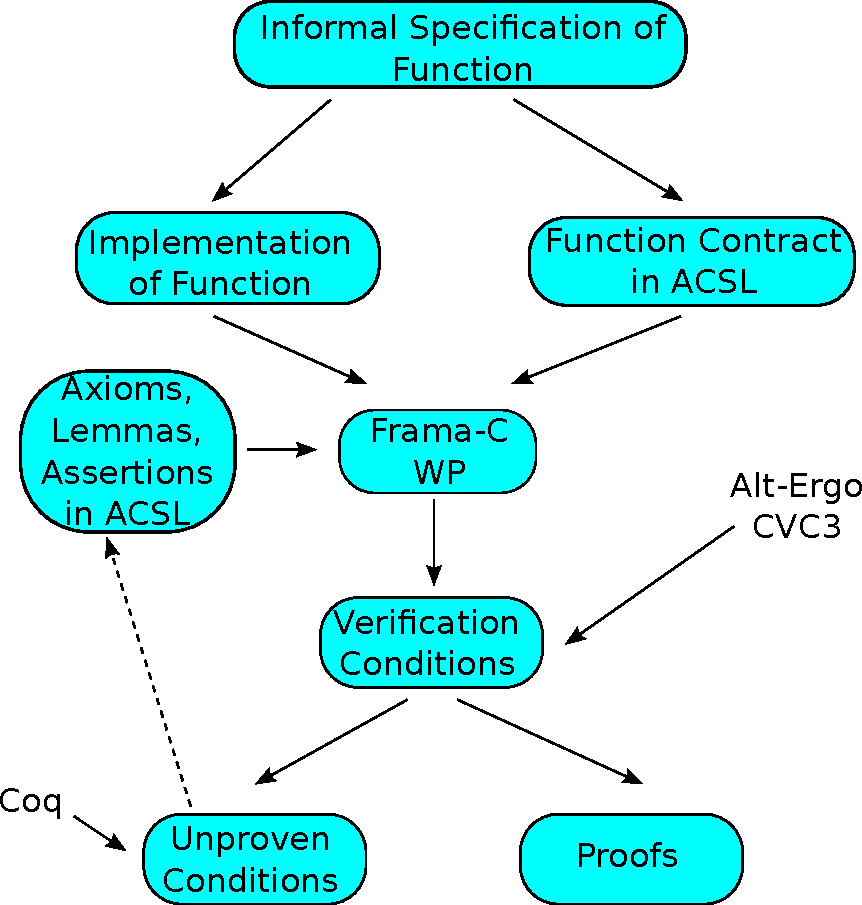
\includegraphics[width=0.60\textwidth]{figures/method-bitwalker.pdf}
\caption{\label{fig:method} The method to formally verify the Bitwalker.}
\end{figure}

Starting point is an informal specification of a function with which in mind
a implementation is written and on which basis the formal specification is created.
The formal specification of a function is a so-called function contract
which contains preconditions to express what a function expects from its caller
and postconditions to state the guarantees after the execution.
The specification language is called 
\acsl (ANSI\slash ISO-\isoc Specification Language)~\cite{acsl} 
which is a formal language to express behavioral properties of \isoc programs.

Moreover, it is the specification language associated with 
the verification platform \framac~\cite{FramaC}
which we use along with its plug-in \wpframac~\cite{wp}.
Within \framac, \wpframac enables the deductive verification of
\isoc programs that have been annotated with \acsl.
\wpframac generates verification conditions which are submitted to external 
automatic or interactive theorem provers.
A function is then verified if each verification condition is discharged
by at least one prover.

Figure~\ref{fig:method} shows that we first apply the automatic
theorem provers \altergo~\cite{alt-ergo} and \cvc~\cite{cvc3}
and then apply the
interactive theorem prover \coq~\cite{Coq}
for the still unproven conditions in order to automate as much as possible.
Moreover, unproven conditions motivate to give some extra information
in the form of axioms, lemmas and assertions in \acsl, 
since they can ease the search of a proof.
One need to be careful with axioms because they can yield contradictions
and thus make the proof system unsound.
This is different for lemmas and assertions
because \wpframac will generate additional verification conditions for them.

In order to prove the absence of run time errors we use
the \inl{rte} option of \wpframac that automatically introduce \acsl
assertions. If all these assertions can be proven, then
the absence of run time errors is guaranteed.


\clearpage

\subsection{The Function \peek}
\label{peek}


In this section we examine the function \peek.
Initially, we provide an informal specification 
followed by an implementation.
We then derive a formal specification on the basis of the informal one. 
Finally, we present the results of the deductive verification with \framac and \wpframac.


\subsubsection{Informal Specification}
\label{informal-peek}


We first introduce some auxiliary concepts and formulate general assumptions:

\begin{itemize}
\item
A \emph{bit stream} is an array containing elements of type \verb"uint8_t".

A bit stream of length $n$ contains $8n$ bits.

\item
A bit stream is \emph{valid} if the array is valid.

\item 
A bit stream can be indexed both by its array indices
and its \emph{bit indices}.

Figure~\ref{fig:bitstream-indices} shows the difference between 
array indices and bit indices in a bit stream.
The two bit indices, 0~and~14,
mark bit positions in the first and second array element, respectively.

\begin{figure}[hbt]
\begin{center}
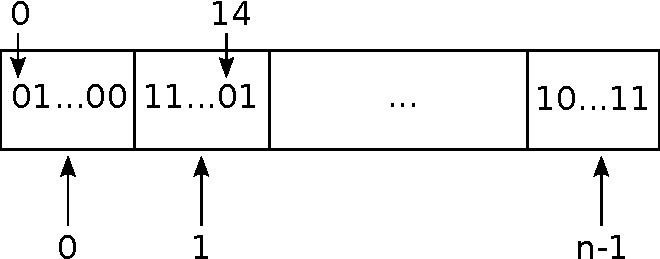
\includegraphics[width=0.40\textwidth]{figures/array_as_stream.pdf}
\caption{\label{fig:bitstream-indices} Array indices and bit indices in a bit stream}
\end{center}
\end{figure}


\item
A \emph{bit sequence} is a consecutive sequence of bits within a bit stream
as represented in Figure~\ref{fig:bitsequence}.
\begin{figure}[hbt]
\begin{center}
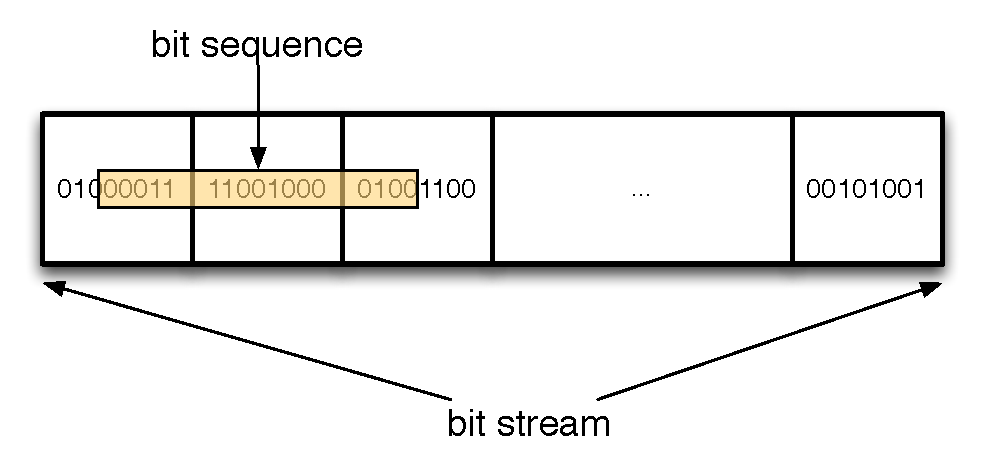
\includegraphics[width=0.40\textwidth]{figures/bit_sequence.pdf}
\caption{\label{fig:bitsequence} A bit sequence within a bit stream}
\end{center}
\end{figure}

A bit sequence is given by the position of its first bit (a bit index in the bit stream)
and its \emph{length}, that is, the number of bits it contains.

\item A bit sequence of length $l$ that starts at bit index $p$ is \emph{valid}
     with respect to a bit stream of length $n$ if the following conditions are
     satisfied
     \begin{align*}
         0 &\leq p \leq 8n \\
         0 &\leq p + l \leq 8n
     \end{align*}

\item 
We assume that the C-types \texttt{unsigned int} and \texttt{int}
have a width of~32~bits.

\end{itemize}

Now we specify \peek with the introduced auxiliary concepts.
The function \texttt{Bitwalker\_Peek} reads a bit sequence from a bit stream
and converts it to an integer.

Its function signature reads as follows:

\begin{lstlisting}[style=acsl-block]
uint64_t  Bitwalker_Peek(unsigned int Startposition, 
                         unsigned int Length,
                         uint8_t Bitstream[],
                         unsigned int BitstreamSizeInBytes);
\end{lstlisting}

The arguments have the following purpose:
\begin{itemize}
    \item \texttt{Startposition} is the bit index in the bit stream 
    where the bit sequence starts.
    \item \texttt{Length} is the length of the bit sequence.
    \item \texttt{Bitstream} is the array which provides the bit stream.
    \item \texttt{BitstreamSizeInBytes} is the length of the array 
    containing the bit stream. 
\end{itemize}


The following preconditions shall hold for the function arguments:
\begin{itemize}
\item \texttt{Bitstream} is a valid array of length \verb"BitstreamSizeInBytes"

\item \texttt{Length} $\leq$ \texttt{64} and

\item \texttt{Startposition + Length} $\leq$ \verb"UINT_MAX".
\end{itemize}

Note that additional constraints are implicitly expressed by the use
of \emph{unsigned} integer types.

We continue with a more precise description of the desired behavior of \peek.
As mentioned, the function \texttt{Bitwalker\_Peek} reads a bit sequence from a bit stream
and converts it to a 64-bit unsigned integer.

The left most bit of the bit sequence is interpreted as
the most significant bit.
Thus, for a bit sequence $(b_0, b_1,\ldots,b_{n - 1})$ the function
returns the sum
\begin{align}
    b_0 \cdot 2^{n - 1} + b_1\cdot 2^{n - 2} + \ldots + b_{n-1}\cdot 2^0
    =
    \sum_{i=0}^{n-1} b_i \cdot 2^{(n - 1) - i} 
\end{align}

If the bit sequence is not valid, then the function returns \texttt{0}.
This increases the robustness of the function.

\clearpage
\subsubsection{Implementation}
\label{impl-peek}
 
Listing~\ref{fig:impl-peek} shows the \isoc implementation of \peek 
for which we aim to verify that it fulfills the informal specification.
The case where the bit sequence is not valid is handled by the \texttt{if}-statement.
For a valid sequence the summation of the bits is done in the \texttt{for}-loop.
The array \texttt{BitwalkerBitMaskTable} is a \texttt{const} helper array 
to select a single bit in the \texttt{Bitstream}.

\begin{listing}[hbt]
\begin{minipage}{\textwidth}
\lstinputlisting[style=acsl-block, frame=single]{./figures/peek.impl}
\end{minipage}
\caption{\label{fig:impl-peek} Implementation of \peek}
\end{listing}

The implementation uses a great amount of bit operations
which is quite a challenge for the formal verification.
We will discuss this further in section~\ref{issues}.

\clearpage

\subsubsection{Formal Specification with \acsl}
\label{formal-peek}

In order to verify that the given implementation of \peek fulfills 
the informal specification, we have to formalize the specification.
Listing~\ref{fig:spec-peek} shows such a formalization in \acsl for \peek.

\begin{listing}[hbt]
\begin{minipage}{\textwidth}
\lstinputlisting[style=acsl-block, frame=single]{./figures/peek.spec}
\end{minipage}
\caption{\label{fig:spec-peek} Formal specification of \peek in \acsl}
\end{listing}

We specify a function contract for \peek containing preconditions
and postconditions introduced by the key words \inl{requires}
and \inl{ensures}, respectively.
In addition, the \acsl language provides the \inl{assigns} clause to specify 
that a function is not allowed to change memory locations other than the ones 
explicitly listed. 
When no \inl{assigns} clauses are specified, 
the function is allowed to modify every visible variable. 

The three preconditions for the function arguments of the informal specification 
are formalized straight forward in the function contract also by three preconditions.
For the first one we use the predicate \inl{IsValidRange}
which we specified in \acsl in order to state that the \inl{Bitstream}
is a valid array of length \inl{BitstreamSizeInBytes}.
Furthermore, we claim that \peek does not alter any memory locations
apart from internal function variables via the \inl{assigns} clause.

Moreover, we use so-called behaviors in \acsl for a distinction of the two cases
from the informal specification.
The cases are discriminated through the predicate \texttt{ValidBitIndex}
which indicates whether a bit sequence is valid or not.
The first behavior \texttt{out\_of\_range} represents the robustness 
case where the bit sequence is not valid and 
the second behavior specifies the expected behavior in the normal case.

In both cases we state what the result of \peek shall be 
as postconditions. In addition, we use a negated form of
a predicate called \inl{TooBig} in the last postcondition of
the normal case. This postcondition was introduced to verify
that the functions \peek and \poke interact correctly.
Therefore, we will discuss this postcondition in section~\ref{interaction}.

Since the implementation of \peek contains a loop,
we need a loop specification containing a variant for the termination
proof and some invariants to enable the automatic theorem provers
to verify the postconditions.
Although this loop specification is important for the verification,
it is not in the sense to formalize the informal specification.

Since we verify the implementation in respect to the formal specification, 
it is crucial that it matches the informal one. 
Therefore, we reviewed the accordance of both specifications.

%\clearpage
\subsubsection{Formal Verification with \framac/\wpframac}
\label{verification-peek}

In this section we present the current state of the verification results 
for \peek.
Table~\ref{tab:results-peek} discriminates the results for
three different types of verification conditions (VCs).

\begin{table}[hbt]
  \centering
  \begin{tabular}[htb]{lccc}
    \toprule
     & \# VC & Proven VCs & Verification rate in \%\\
    \midrule
    lemmas & $1$ &$0$ & $0$ \\
    %\midrule
    rte-assertions&$9$&$5$&$55$\\
    rest &$18$ &$17$&$94$\\
 %   \bottomrule
%    &$27$&$22$&$81$\\
    \bottomrule
  \end{tabular}
  \caption{Verification Results of \peek}
  \label{tab:results-peek}
\end{table}


The first row contains the lemmas we used to ease the verification for the automatic theorem provers.
While the second row contains the \inl{rte}-assertions 
concerning the absence of run time errors.
The third row shows all other verification conditions for \peek
which are mainly about for correct functional behavior.
However, they also contain the postconditions for the robustness cases
and the loop specification.

For each row we listed the total number of generated verification conditions,
the number of proven verification conditions and the verification rate
that is the percentage of proven verification conditions. 

The verification rate for the \inl{rte}-assertions are very low 
due to the difficulty for \framac to deal with bit operations.
In order to increase this rate, we will verify the absence
of run time errors separately and will provide additional lemmas and axioms
to ease the verification.
We point out some of the related challenges in section~\ref{issues}.



\clearpage

\subsection{The Function \poke}
\label{poke}


In this section we examine the function \poke
in the same manner as we did it for \peek in section~\ref{peek}.

\subsubsection{Informal Specification}
\label{informal-poke}

The function \poke converts an integer to a bit sequence and writes it
into a bit stream.
Its function signature reads as follows:
\begin{lstlisting}[style = acsl-block]
int      Bitwalker_Poke(unsigned int Startposition,
                        unsigned int Length,
                        uint8_t Bitstream[],
                        unsigned int BitstreamSizeInBytes,
                        uint64_t Value);
\end{lstlisting}


%\subsubsection*{Arguments}
The arguments have the following purpose:

\begin{itemize}
    \item \texttt{Startposition} is the bit index in the bit stream 
    where the bit sequence starts.
    \item \texttt{Length} is the length of the bit sequence.
    \item \texttt{Bitstream} is the array which provides the bit stream.
    \item \texttt{BitstreamSizeInBytes} is the length of the array 
    containing the bit stream. 
    \item \texttt{Value} is the integer which shall be converted into a bit sequence.
\end{itemize}


%\subsubsection*{Preconditions}
The following preconditions shall hold for the function arguments:

\begin{itemize}
\item \texttt{Bitstream} is a valid array of length \verb"BitstreamSizeInBytes"

\item \texttt{Length} $<$ \texttt{unsigned int}.

\item \texttt{Startposition + Length} $\leq$ \verb"UINT_MAX".
\end{itemize}

Note that additional constraints are implicitly expressed by the use
of \emph{unsigned} integer types.


%\subsubsection*{Description}
Now we can specify \poke as follows:
The function \poke converts a 64-bit unsigned integer to a bit sequence and 
writes it into a bit stream.

For $0 \leq x$ exists a shortest sequence of~0 and~1
$(b_0, b_1,\ldots,b_{n - 1})$
such that
\begin{align}
    \sum_{i=0}^{n-1} b_i \cdot 2^{(n - 1) - i} = x.
\end{align}

The function \poke tries to store the sequence $(b_0, b_1,\ldots,b_{n - 1})$
in the bit sequence of \texttt{Length} bits that starts
at bit index \texttt{Startposition}.

The return value of \poke depends on the following three cases:

\begin{itemize}
\item 
If the bit sequence is valid, then there are two cases:

\begin{itemize}
\item
If $\texttt{Length} \geq n$, then  the sequence
$(\overbrace{0,\ldots,0}^{\texttt{Length}-n},b_0, b_1,\ldots,b_{n - 1})$
is stored in the bit stream starting at \texttt{Startposition}.
The return value of \poke is 0.

\item
If $\texttt{Length} < n$, then the
sequence $(b_0, b_1,\ldots,b_{n - 1})$ cannot be stored and\\
\poke returns~$-2$.
\end{itemize}

\item 
If the bit sequence is not valid, then \poke returns~$-1$.
\end{itemize}

\subsubsection{Implementation}
\label{impl-poke}
Listing \ref{fig:impl-poke} shows the implementation of \poke
which discriminates three cases. The first two are the robustness cases
of the informal specification and the last one is
the normal case where the function actually writes into the bit stream.
Similar to \peek a lot of bit operations are used. 

\begin{listing}[hbt]
\begin{minipage}{\textwidth}
\lstinputlisting[style=acsl-block, frame=single]{./figures/poke.impl}
\end{minipage}
\caption{\label{fig:impl-poke} Implementation of \poke}
\end{listing}



\clearpage
\subsubsection{Formal Specification with ACSL}
\label{formal-poke}

Listing~\ref{fig:spec-poke} shows the function contract of \poke.
The case independent preconditions of the informal specification 
are reflected by the  first three \inl{requires}-clauses at the beginning of the contract.
\poke modifies the \inl{Bitstream} and reads the array
\inl{BitwalkerBitMaskTable} thus we need to express 
that the two arrays must have separated memory locations. 
Therefore, we use the predicate \inl{separated} in the fourth \inl{requires}-clause.
Furthermore, in the following \inl{assigns}-clause we specify the memory locations which 
can be altered by the function.

We specify the three cases of \poke by using behaviors. 
The first behavior \inl{out\_of\_range} occurs if the given bit sequence is not valid with respect to the \inl{Bitstream}. 
The second behavior \inl{value\_too\_big} covers the case that the value \inl{Value} 
is not representable with only \inl{Length} bits.

Finally, the behavior \inl{normal} assumes 
that \inl{Value} is not too big and the bit sequence is valid. 
Here, \poke writes the particular bit sequence into \inl{Bitstream} 
while all other memory locations are unaltered.
For all behaviors there is one postcondition to state what
the return value shall be in this case.


\begin{listing}[hbt]
\begin{minipage}{\textwidth}
\lstinputlisting[style=acsl-block, frame=single]{./figures/poke.spec}
\end{minipage}
\caption{\label{fig:spec-poke} Formal Specification of \poke}
\end{listing}



\FloatBarrier

\subsubsection{Formal Verification with Frama-C/WP}
\label{verification-poke}

In this section we present the current state of verification results of 
for \poke.
The results are shown in Table~\ref{tab:results-poke}.
 We listed the different verification conditions 
 row by row like we did it for \peek.

The function \poke has significantly more unproven verification conditions than \peek
this is because it is more complex and alters memory locations via bit operations.
Therefore, we will verify the absence of run time errors separately as well.

\begin{table}[hbt]
  \centering
  \begin{tabular}[h]{lccc}
    \toprule
     & \# VC & Proven VCs & Proven VCs in \%\\
    \midrule
    lemmas & $1$ &$0$ & $0$ \\
    %\midrule
    rte-assertions&$19$&$7$&$36$\\
    rest &$49$ &$38$&$77$\\
    %\bottomrule
    %&$68$&$45$&$66$\\
    \bottomrule
  \end{tabular}
  \caption{Verification Results of \poke}
  \label{tab:results-poke}
\end{table}



\clearpage
\subsection{Interaction of \peek and \poke}
\label{interaction}


In this section we examine the interaction of 
\peek and \poke. The functions shall be inverse to each other
in respect to the normal cases of both functions.
In the following we provide a formal specification and present
our verification results.


\subsubsection{Formal Specification with ACSL and C}

For the specification of the interaction we have two auxiliary \isoc functions:
The first one to call first \poke on a bit stream and then \peek
and the second one to do it the other way around.

Figure~\ref{fig:poke-peek} shows the straight forward implementation 
of the first helper function along with its \acsl contract.
The contract contains a lot of preconditions because we
only specify an interaction for the case that both functions are in their normal
cases. The reader can compare the preconditions with them from
the contracts of \peek and \poke with respect to the \inl{normal} behaviors.
As a postcondition we formulate that \peek reads exactly the value
written by \poke.

\begin{listing}[hbt]
\begin{minipage}{\textwidth}
\lstinputlisting[style=acsl-block, frame=single, linerange=3-20]{./figures/Peek_Poke_inverse.c}
\end{minipage}
\caption{\label{fig:poke-peek} Specification of interaction when first calling \poke.}
\end{listing}

Figure~\ref{fig:peek-poke} shows the straight forward implementation 
of the second auxiliary function along with its \acsl contract.
In contrast to the first function, we work with two bit streams.
With \peek a certain bit sequence is read out from one bit stream
and written via \poke into the other one.
Therefore, we formulate as a postconditions that
the two bit streams are equal in these certain ranges.

\begin{listing}[hbt]
\begin{minipage}{\textwidth}
\lstinputlisting[style=acsl-block, frame=single, linerange=22-43]{./figures/Peek_Poke_inverse.c}
\end{minipage}
\caption{\label{fig:peek-poke} Specification of interaction when first calling \peek.}
\end{listing}

 \FloatBarrier

\subsubsection{Formal Verification with Frama-C/WP}

All postconditions (and the assertion in figure~\ref{fig:peek-poke})
are verified. Therefore, we succeeded to prove that the 
functions \peek and \poke interact correctly
in respect to their specifications.

Moreover, this verification result serves as a validation for the contracts
of \peek and \poke because the verification of the interaction 
depends on these contracts. Since both functions are called,
the caller has to assure that all preconditions hold
and can then rely on the guarantees given by the postconditions.

As a remark, we extended the contract of \peek by one postcondition 
to ease the verification of the interaction.
The postcondition simply states that the read value is always representable 
by \inl{Length} bits which is obviously always the case,
since the value is the sum of \inl{Length} bits.
The postcondition is needed to assure that the preconditions for the normal case
of \poke are fulfilled when first calling \peek and then \poke.

\clearpage

\subsection{Open Issues}
\label{issues}


We have seen in this section that \wpframac currently does not deal very well with bit operations.
This is due to the fact that \wpframac's memory models do not provide 
much information about bit operations.
As a consequence, the provers have few options to manipulate the proof goal.
This problem is known and \cealist is working on a solution for the next release of \wpframac.

As a workaround one could introduce axioms which provide
additional facts about bit operations. 
The problem with using axioms is that one can easily introduce wrong facts
which lead to contradictions  that make the whole proof system unsound. 
Thus, this approach requires a careful review of the added axioms.

Moreover, the chosen automatic theorem provers are generally not very
good when it comes to mixing arithmetic and bit operations.
There is, however, an automatic theorem prover, namely \z,
which can handle arithmetic and bit operations.
\framac does currently not provide an interface for \z but this may change in a future release.
We therefore expect a better automatic verification rate for the verification of BitWalker.

Another approach to deal with unproven verification conditions consists in
applying an \emph{interactive theorem prover} such as \coq.
Using \coq's rich support for proof manipulation would certainly be very helpful
for the discharge of more proof obligations.

\clearpage

\section{SQS}
\label{sec:sqs}

\subsection{Introduction}
In this section we describe our work on the static code analysis of the bitwalker code provided in \href{https://github.com/openETCS/validation/tree/master/Artifacts/Subset-026-7_XML/Subset026_7/Bitwalker}{[validation repository]}

Our aim is to discover programing errors, obtain code metrics (lines of code, lines of code/lines of comments, cyclomatic complexity, class inherance tree and others) and verify some subset of rules defined in the MISRA C Standard.

The code metrics help understanding the complexity of the code and can lead to code changes. For
example, the cyclomatic complexity or the number of paths, are a precise measure of the code complexity, and the more complex the code is, more likely it will contain masked bugs.

Five different static analysis tools have been used during the code verification activities in order to assess the quality of the results and ensure code quality.

Finally, according to the results obtained by using the tools, we will present some conclusions.

\subsection{Resource Standard Metrics -RSM- Results}
In this section we provide the results obtained with the RSM tool.

Resource Standard Metrics (RSM) is a source code metrics and quality analysis tool.

RSM provides standard metrics and a combination of features that allow to:
\begin{itemize}
\item Analyze source code for programming errors
\item Analyze source code for code style enforcement
\item Create an Inheritance tree from the code
\item Collect Source Code Metrics by the function, class, file, and project
\item Analyze Cyclomatic Complexity
\end{itemize}

Furthermore, RSM tool is mapped to the \href{http://msquaredtechnologies.com/m2rsm/docs/QualityStandards/MISRA_C_Mapping.htm}{[MISRA C]} Industry Standards which coverage is 40.16\% 


Besides, RSM has intrinsic quality notices and can be extended by the end user with User Defined Quality Notices using regular expressions to analyze code lines. 

The following table shows the intrinsic Quality Notices for language c that RSM tool checks.

{\footnotesize\sffamily\centering
  \begin{longtable}{||p{.45\textwidth}|p{.5\textwidth}||}
  \caption{Quality Notices}\\
    \hline\hline
    \hline\hline
    \endhead
    \hline\hline
    \endfoot
    \textbf{Quality Notice No. 1}

Emit a quality notice when the physical line length is greater than the specified number of characters.

Rationale:  \textcolor{red}{Reproducing source code on devices that are limited to 80 columns of text can cause the truncation of the line or wrap the line.  Wrapped source lines are difficult to read, thus creating weaker peer reviews of the source code}.
& \textbf{Quality Notice No. 2}

Emit a quality notice when the function name length is greater than the specified number of characters.  

Rationale:  \textcolor{red}{Long function names may be a portability issue especially when code has to be cross compiled onto embedded platforms.  This difficultly is typically seen with older hardware and operating systems.}
    \\
    \hline \textbf{Quality Notice No. 3}
    
Emit a quality notice when ellipsis '...' are identified within a functions parameter list thus enabling variable arguments.  

Rationale:  \textcolor{red}{Ellipsis create a variable argument list.  This type of design is found in C and C++.  It essentially breaks the type strict nature of C++ and should be avoided.}
 & \textbf{Quality Notice No. 4}
 
Emit a quality notice if there exists an assignment
operator '=' within a logical 'if' condition.

Rationale:  \textcolor{red}{An assignment within an "if" condition is likely a typographical error giving rise to a logic defect.  However, some programmers place compound statements into the "if" condition making the code difficult to read.}
    \\
    \hline \textbf{Quality Notice No. 5}
    
Emit a quality notice if there exists an assignment
operator '=' within a logical 'while' condition.

Rationale:  \textcolor{red}{An assignment within a "while" condition is likely a typographical error giving rise to a logic defect.  However, some programmers place compound statements into the "while" condition making the code difficult to read.}
 & \textbf{Quality Notice No. 6}
 
Emit a quality notice when a pre-decrement operator '--' is identified within the code.  

Rationale: \textcolor{red}{ The pre-decrement of a variable occurs before the remainder of the processing in the statement.  This can be difficult to comprehend or anticipate.  There are documented cases where the mathematical results vary between the result of macros when different code preprocessors expand the macros into a normal form.  Remember, there is no standard for the preprocessor, just the language.}
    \\
    \hline \textbf{Quality Notice No. 7}
    
Emit a quality notice when a pre-increment operator '++' is identified within the code.

Rationale:  \textcolor{red}{The pre-increment of a variable occurs before the remainder of the processing in the statement.  This can be difficult to comprehend or anticipate.  There are documented cases where the mathematical results vary between the result of macros when different code preprocessors expand the macros into a normal form.}  
& \textbf{Quality Notice No. 8}

Emit a quality notice when the 'realloc' function
is identified within the code.

Rationale:  \textcolor{red}{Using realloc can lead to latent memory leaks within your C or C++ code.  The call to realloc reassigns the pointer to the same memory address using a larger or smaller space.  However if realloc fails, a NULL pointer is returned.  No "free" was performed on the pointer so if you don't retain the pointer before the realloc call, a latent memory leak could occur.}
    \\
    \hline \textbf{Quality Notice No. 9}
    
Emit a quality notice when the 'goto' function
is identified within the code.

Rationale:  \textcolor{red}{The use of "goto" creates spaghetti code.  A "goto" can jump anywhere to the destination label.  This type of design breaks the "one in - one out" ideal of a function creating code which can be impossible to debug or maintain.}
 & \textbf{Quality Notice No. 10}
 
Emit a quality notice when the Non-ANSI function prototype is identified within the code.

Rationale:  \textcolor{red}{Older C code can be written in a style that does not use function prototypes of the function argument types.  This code will not compile on ANSI C and C++ compilers because of this type of weakness.  Identifying this condition can help assess whether code can be ported to a newer version of the language.}
    \\
    \hline \textbf{Quality Notice No. 11}
    
Emit a quality notice when open and closed brackets '[ ]' are not balance within a file.

Rationale:  \textcolor{red}{This type of error is always caught by the compiler as a syntax error.  However, a compiler can be told to ignore source code by using preprocessor directives like \#if ... \#endif.  This is a way to "comment" out large blocks of code.  However, the code still looks like operational code to the maintainer as it is not a comment.  Many hours can be wasted working on dead code.  This quality notice serves to warn you of this dead code that should be removed or converted to actual comment form.}
 & \textbf{Quality Notice No. 12}
 
Emit a quality notice when open and closed parenthesis '( )' are not balance within a file.

Rationale:  \textcolor{red}{This type of error is always caught by the compiler as a syntax error.  However, a compiler can be told to ignore source code by using preprocessor directives like \#if ... \#endif.  This is a way to "comment" out large blocks of code.  However, the code still looks like operational code to the maintainer as it is not a comment.  Many hours can be wasted working on dead code.  This quality notice serves to warn you of this dead code that should be removed or converted to actual comment form.}.
    \\
    \hline \textbf{Quality Notice No. 13}
    
Emit a quality notice when a 'switch' statement does not have a 'default' condition.

Rationale:  \textcolor{red}{A "switch" statement must always have a default condition or this logic construct is non-deterministic.  Generally the default condition should warn the user of an anomalous condition which was not anticipated by the programmer by the case clauses of the switch.}
 & \textbf{Quality Notice No. 14}
 
Emit a quality notice when there are more 'case' conditions than 'break', 'return' or 'fall through' comments.

Rationale:  \textcolor{red}{Many tools, including RSM, watch the use of "case" and "break" to insure that there is not an inadvertent fall through to the next case statement.  RSM requires the programmer to explicitly indicate in the source code via a "fall through" comment that the case was designed to fall through to the next statement.}
    \\
    \hline \textbf{Quality Notice No. 16}
    
Emit a quality notice when function white space
percentage is less than the specified minimum.

Rational:  \textcolor{red}{Source code must be easily read.  A low percentage of white space indicates that the source code is crammed together thus compromising the readability of the code.  Typically white space less than 10 percent is considered crammed  code. }
 & \textbf{Quality Notice No. 17}
 
Emit a quality notice when function comment
percentage is less than the specified minimum.

Rationale:  \textcolor{red}{A programmer must supply sufficient comments to enable the understandability of the source code.  Typically a comment percentage less than 10 percent is considered insufficient.  However, the content quality of the comment is just as important as the quantity of the comments.  For this reason you could use the -E option to extract all the comments from a file.  The reviewer should be able to read the comments and extract the story of the code.}
    \\
    \hline \textbf{Quality Notice No. 18}
    
Emit a quality notice when the eLOC within a
function exceeds the specified maximum.

Rationale:  \textcolor{red}{An extremely large function is very difficult to maintain and understand.  When a function exceeds 200 eLOC (effective lines of code), it typically indicates that the function could be broken down into several functions.  Small modules are desirable for modular composability.}
 & \textbf{Quality Notice No. 19}
 
Emit a quality notice when file white space
percentage is less than the specified minimum.

Rationale:  \textcolor{red}{Source code must be easily read.  A low percentage of white space indicates that the source code is crammed together thus compromising the readability of the code.  Typically white space less than 10 percent is considered crammed  code.}

    \\
    \hline \textbf{Quality Notice No. 20}
    
Emit a quality notice when file comment
percentage is less than the specified minimum.

Rationale:  \textcolor{red}{A programmer must supply sufficient comments to enable the understandability of the source code.  Typically a comment percentage less than 10 percent is considered insufficient.  However, the content quality of the comment is just as important as the quantity of the comments.  For this reason you could use the -E option to extract all the comments from a file.  The reviewer should be able to read the comments and extract the story of the code.}
 & \textbf{Quality Notice No. 22}
 
Emit a quality notice when each if, else, for
or while is not bound by scope.

Rationale:  \textcolor{red}{Logical blocks should be bound with scope.  This clearly marks the boundaries of scope for the logical blocks.  Many times, code may be added to non-scoped logic blocks thus pushing other lines of code from the active region of the logical construct giving rise to a logic defect.}
    \\
    \hline 
    \textbf{Quality Notice No. 23}
    
Emit a quality notice when the '?' or the implied
if-then-else construct has been identified.

Rationale:  \textcolor{red}{The ? operator creates the code equivalent of an "if" then "else" construct.  However the resultant source is far less readable.}
 & \textbf{Quality Notice No. 24}
 
Emit a quality notice when an ANSI C++ keyword is identified within a *.c or a *.h file.

Rationale: \textcolor{red}{ In C source code it is possible to find variable names like "class".  This word is a key word in C++ and would prevent this C code from being ported to the C++ language.}
    \\
    \hline
\textbf{Quality Notice No. 25} (Deprecated RSM 6.70) 

When analyzing *.h files for C++ keywords,
assume that *.h can be both C and C++.

Rationale: \textcolor{red}{ A *.h file can be either a C or C++ source file.  If a *.h file is assumed to be from either language, then RSM will not emit C keyword notices in *.h file, only for *.c files.}
 & \textbf{Quality Notice No. 26}
 
Emit a quality notice when a void * is identified
within a source file.

Rationale:  \textcolor{red}{A "void *" is a type-less pointer.  ANSI C and C++ strives to be type strict.  In C++ a "void *" breaks the type strict nature of the language which can give rise to anomalous run-time defects.}
    \\
    \hline
    \textbf{Quality Notice No. 27}
    
Emit a quality notice when the number of function return points is greater than the specified maximum.

Rationale:  \textcolor{red}{A well constructed function has one entry point and one exit point.  Functions with multiple return points are difficult to debug and maintain.}
 & \textbf{Quality Notice No. 28}
 
Emit a quality notice when the cyclomatic complexity of a function exceeds the specified maximum.

Rationale:  \textcolor{red}{Cyclomatic complexity is an indicator for the number of logical branches within a function.  A high degree of V(g), greater than 10 or 20, indicates that the function could be broken down into a more modular design of smaller functions.}
    \\
    \hline
        \textbf{Quality Notice No. 29}
        
Emit a quality notice when the number of function input parameters exceeds the specified maximum.

Rationale:  \textcolor{red}{A high number of input parameters to a function indicates poor modular design.  Data should be grouped into representative data types.  Functions should be specific to one purpose.}
 & \textbf{Quality Notice No. 30}
 
Emit a quality notice when a TAB character is identified within the source code. Indentation with TAB will create editor and device dependent formatting.

Rationale:  \textcolor{red}{Tab characters within source code create documents that are print and display device dependent.  The document may look correct on the screen but it may become unreadable when printed.}
    \\
    \hline
        \textbf{Quality Notice No. 31}
        
Emit a quality notice when class comment
percentage is less than the specified minimum.

Rationale:  \textcolor{red}{A programmer must supply sufficient comments to enable the understandability of the source code.  Typically a comment percentage less than 10 percent is considered insufficient.}
 & \textbf{Quality Notice No. 43}
 
Emit a quality notice when the key word 'continue' has been identified within the source code.

Rationale:  \textcolor{red}{The use of 'continue' in logical structures causes a disruption in the linear flow of the logic.  This style of  programming can make maintenance and readability difficult.}
    \\
    \hline
        \textbf{Quality Notice No. 46}
        
Emit a quality notice when function, struct, class or interface blank line percentages are less than the specified minimum
 
Rationale:  \textcolor{red}{The amount of blank lines in a file can indicate the degree of readability in the file. It indicates the author intended his work to be human consumable.}
 & \textbf{Quality Notice No. 47}
 
Emit a quality notice when the file blank line percentage is less than the specified minimum

Rationale: \textcolor{red}{The amount of blank lines in a file can indicate the degree of readability in the file. It indicates the author indented his work to be human consumable.}
    \\
    \hline
        \textbf{Quality Notice No. 48}
        
Emit a quality notice when a function has no logical lines of code. 
 
Rationale: \textcolor{red}{This condition indicates a no-op or stubbed out function with no operational code.Many code generators create such no-op functions which contribute to code bloat and unnecessary resource utilization.}
 & \textbf{Quality Notice No. 49}
 
Emit a quality notice when a function has no parameters in the parameter list.

Rationale:  \textcolor{red}{A function should always specify the actual parameter names to enhance maintenance and readability. A programmer should always put void to indicate the deliberate design in the code.}
    \\
    \hline
        \textbf{Quality Notice No. 50}
         
Emit a quality notice when a variable is assigned to a literal value. Configurable for literal 0 in rsm.cfg. 

Rationale: \textcolor{red}{A symbolic constant is the preferred method for variable assignment as this creates maintainable and understandable.}
 & \textbf{Quality Notice No. 51}
 
Emit a quality notice when there is no comment before a function block. 
 
Rationale: \textcolor{red}{A function block should retain a preceding comment block describing the purpose, parameters, returns and algorithms.}
    \\
    \hline
     \textbf{Quality Notice No. 52}
     
Emit a quality notice when there is no comment before a class block. 
 
Rationale: \textcolor{red}{A class block should retain a preceding comment block describing the purpose, and algorithms.}
 & \textbf{Quality Notice No. 53}
 
Emit a quality notice when there is no comment before a struct block. 

Rationale: \textcolor{red}{A struct block should retain a preceding comment block describing the data and purpose.}
    \\
    \hline
     \textbf{Quality Notice No. 55}
     
Emit a quality notice when scope exceeds the specified maximum in the rsm.cfg file. 
 
Rationale: \textcolor{red}{A deep scope block of complex logic or levels may indicate a maintenance concern.}
 & \textbf{Quality Notice No. 56}
 
Emit a quality notice when sequential break statements are identified.

Rationale: \textcolor{red}{Repetitive and sequential breaks can be used to fool RSM identification of case statement without breaks.}
    \\
    \hline
\end{longtable}}

In addition to this, RSM allows to customize the desired output providing standard metrics
and a combination of features.

RSM has been customized to obtain the below metrics and analysis and the corresponding reports that are available into the \href{https://github.com/openETCS/validation/tree/master/VnVUserStories/VnVUserStorySQS/04-Results}{[VnVUserStories folder]}

\begin{itemize}
\item Project Functional Metrics and Analysis
\item Project Class/Struct Metrics and Analysis
\item Class Inheritance Tree
\item Project Quality Profile
\item Quality Notice Density
\item Files Keywords and Metrics
\item Project Keywords and Metrics
\item Files Function Metrics
\item Class/Struct Metrics
\item Complexity Metrics
\end{itemize}

At following we provide a summary of the obtained results.

The table below indicates the total quality profile (Summary by notice type) for the bitwalker code which result is especially useful for determining the overall internal code quality.
         
           
\begin{longtable}{||p{.1\textwidth}|p{.1\textwidth}|p{.1\textwidth}|p{.6\textwidth}||}
  \caption{Quality Profile}\\
    \hline\hline
    \textbf{Type} & \textbf{Count} & \textbf{Percent} & \textbf{Quality Notice} \\
    \hline\hline
    \endhead
    \hline\hline
    \endfoot
    \textcolor{red}{1} & \textcolor{blue}{38}
& 9.57
& Physical line length > 80 characters
    \\
    \hline
    \textcolor{red}{2} & \textcolor{blue}{4}
& 1.01
& Function name length > 32 characters
    \\
    \hline
    \textcolor{red}{22} & \textcolor{blue}{5}
& 1.26
& if, else, for or while not bound by scope
    \\
    \hline
    \textcolor{red}{27} & \textcolor{blue}{2}
& 0.50
& Number of function return points > 1
    \\
    \hline
    \textcolor{red}{30} & \textcolor{blue}{330}
& 83.12
& TAB character has been identified
    \\
    \hline
    \textcolor{red}{50} & \textcolor{blue}{7}
& 1.76
& Variable assignment to a literal number
    \\
    \hline
    \textcolor{red}{51} & \textcolor{blue}{8}
& 2.02
& No comment preceding a function block
    \\
    \hline
    \textcolor{red}{53} & \textcolor{blue}{1}
& 0.25
& No comment preceding a struct block
    \\
    \hline
    \textcolor{red}{125} & \textcolor{blue}{2}
& 0.50
& A data member in the header file is not of the form m\_*
    \\
    \hline
\end{longtable}

The following table shows some code metrics by file.

\begin{longtable}{||p{.275\textwidth}|p{.125\textwidth}|p{.125\textwidth}|p{.075\textwidth}|p{.125\textwidth}|p{.125\textwidth}||}
  \caption{File Summary}\\
    \hline\hline
    \textbf{Metrics} & \textbf{Bitwalker.h} & \textbf{Bitwalker.c} & \textbf{main.c} & \textbf{opnETCS.h} & \textbf{opnETCS \_Decoder.h}\\
    \hline\hline
    \endhead
    \hline\hline
    \endfoot
    \ LOC & 15
& 58
& 45 & 884 & 62
    \\
    \hline
    \ eLOC & 15
& 40
& 40 & 823 & 62
    \\
    \hline
    \ lLOC & 11
& 28
& 23 & 760 & 61
    \\
    \hline
    \ Comment & 16
& 29
& 61 & 822 & 15
    \\
    \hline
    \ Lines & 41
& 109
& 127 & 1249 & 84
    \\
    \hline
   \end{longtable}

Below table provide information regarding standard functional metrics as cyclomatic complexity and others.

The result obtained in the calculation of the cyclomatic complexity defines the number of independent paths within a piece of code and determines the upper bound on the number of tests that must be performed to ensure that each statement is executed at least once.

Taking into account the obtained cyclomatic complexity, the risk can be determined due to McCabe found that a value of 10 is a practical upper limit to the size of a module. When the complexity exceeds this value becomes very difficult to prove, understand and modify it. However, in some circumstances, it may be appropriate to relax the restriction and permit modules with a complexity as high as 15.

\begin{longtable}{||p{.275\textwidth}|p{.125\textwidth}|p{.125\textwidth}|p{.075\textwidth}|p{.125\textwidth}|p{.125\textwidth}||}
  \caption{Functional Summary}\\
    \hline\hline
    \textbf{Metrics} & \textbf{Bitwalker.c} & \textbf{main.c}\\
    \hline\hline
    \endhead
    \hline\hline
    \endfoot
    \ File Function Count
& 7
& 1
    \\
    \hline
    \ Total Function LOC
& 49
& 40
    \\
    \hline
    \ Total Function eLOC
& 31
& 35
    \\
    \hline
    \ Total Function lLOC
& 27
& 23
    \\
    \hline
    \ Total Function Params
& 20
& 0
    \\
    \hline
    \ Total Cyclo Complexity
& 13
& 1
    \\
    \hline
    \ Total Function Pts LOC
& 0.5
& 0.4
    \\
    \hline
    \ Total Function Pts eLOC
& 0.3
& 0.3
    \\
    \hline
    \ Total Function Pts lLOC
& 0.2
& 0.2
    \\
    \hline
    \ Total Function Return
& 10
& 1
    \\
    \hline
    \ Total Function Complex
& 43
& 2
    \\
    \hline
    \ Max Function LOC
& 16
& 40
    \\
    \hline
    \ Max Function eLOC
& 12
& 35
    \\
    \hline
    \ Max Function lLOC
& 9
& 23
    \\
    \hline
    \ Average Function LOC
& 7.00
& 40
    \\
    \hline
    \ Average Function eLOC
& 4.43
& 35
    \\
    \hline
    \ Average Function lLOC
& 3.86
& 23
    \\
    \hline
    \ Max Function Parameters
& 5
& 0
    \\
    \hline
    \ Max Function Returns
& 3
& 1
    \\
    \hline
    \ Max Interface Complex
& 8
& 1
    \\
    \hline
    \ Max Cyclomatic Complex
& 5
& 1
    \\
    \hline
    \ Max Total Complexity
& 13
& 2
    \\
    \hline
    \ Avg Function Parameters
& 2.86
& 0.00
    \\
    \hline
    \ Avg Function Returns
& 1.43
& 1.00
    \\
    \hline
    \ Avg Interface Complex
& 4.29
& 1.00
    \\
    \hline
    \ Avg Cyclomatic Complex
& 1.86
& 1.00
    \\
    \hline
    \ Avg Total Complexity
& 6.14
& 2.00
    \\
    \hline
\end{longtable}

We continue with a more detailed Complexity analysis per function.

\begin{longtable}{||p{.125\textwidth}|p{.125\textwidth}|p{.175\textwidth}|p{.175\textwidth}||}
  \caption{Function Metrics}\\
    \hline\hline
    \endhead
    \hline\hline
    \endfoot
\multicolumn{4}{||l||}{\textbf{Bitwalker\_Peek}}
\\\hline
\multicolumn{4}{||l||}{Cyclomatic Complexity Vg Detail:}
\\\hline
\multicolumn{3}{||c|}{Function Base} & 1
\\\hline
\multicolumn{3}{||c|}{Loops for / foreach} & 1
\\\hline
\multicolumn{3}{||c|}{Conditional if / else if} & 1
\\\hline
\ Param: 4 &
Return: 2 &
Cyclo Vg: 3 &
Comment: 5
 \\\hline
\ LOC: 12 &
eLOC: 8 &
lLOC: 7 &
Lines: 19
 \\\hline
\multicolumn{4}{||l||}{\textbf{Bitwalker\_Poke}}
\\\hline
\multicolumn{4}{||l||}{Cyclomatic Complexity Vg Detail:}
\\\hline
\multicolumn{3}{||c|}{Function Base} & 1
\\\hline
\multicolumn{3}{||c|}{Loops for / foreach} & 1
\\\hline
\multicolumn{3}{||c|}{Conditional if / else if} & 3
\\\hline
\ Param: 5 &
Return: 3 &
Cyclo Vg: 5 &
Comment: 6
 \\\hline
\ LOC: 16 &
eLOC: 12 &
lLOC: 9 &
Lines: 23
 \\\hline
\multicolumn{4}{||l||}{\textbf{Bitwalker\_IncrementalWalker\_Init}}
\\\hline
\ Param: 4 &
Return: 1 &
Cyclo Vg: 1 &
Comment: 0
 \\\hline
\ LOC: 5 &
eLOC: 3 &
lLOC: 3 &
Lines: 5
 \\\hline
\multicolumn{4}{||l||}{\textbf{Bitwalker\_IncrementalWalker\_Peek\_Next}}
\\\hline
\ Param: 2 &
Return: 1 &
Cyclo Vg: 1 &
Comment: 1
 \\\hline
\ LOC: 5 &
eLOC: 3 &
lLOC: 3 &
Lines: 6
 \\\hline
\multicolumn{4}{||l||}{\textbf{Bitwalker\_IncrementalWalker\_Peek\_Finish}}
\\\hline
\ Param: 1 &
Return: 1 &
Cyclo Vg: 1 &
Comment: 0
 \\\hline
\ LOC: 3 &
eLOC: 1 &
lLOC: 1 &
Lines: 3
 \\\hline
\multicolumn{4}{||l||}{\textbf{Bitwalker\_IncrementalWalker\_Poke\_Next}}
\\\hline
\ Param: 3 &
Return: 1 &
Cyclo Vg: 1 &
Comment: 1
 \\\hline
\ LOC: 5 &
eLOC: 3 &
lLOC: 3 &
Lines: 6
 \\\hline
\multicolumn{4}{||l||}{\textbf{Bitwalker\_IncrementalWalker\_Poke\_Finish}}
\\\hline
\ Param: 1 &
Return: 1 &
Cyclo Vg: 1 &
Comment: 0
 \\\hline
\ LOC: 3 &
eLOC: 1 &
lLOC: 1 &
Lines: 3
 \\\hline
\multicolumn{4}{||l||}{\textbf{main}}
\\\hline
\ Param: 0 &
Return: 1 &
Cyclo Vg: 1 &
Comment: 47
 \\\hline
\ LOC: 40 &
eLOC: 35 &
lLOC: 23 &
Lines: 101
 \\\hline
\end{longtable}


\subsection{LocMetrics tool Results}

LocMetrics counts total lines of code (LOC), blank lines of code (BLOC), comment lines of code (CLOC), lines with both code and comments (C\&SLOC), logical source lines of code (SLOC-L), McCabe VG complexity (MVG), Header Comments (HCLOC), Header Words (HCWORD) and number of comment words (CWORDS). Physical executable source lines of code (SLOC-P) is calculated as the total lines of source code minus blank lines and comment lines. Counts are calculated on a per file basis and accumulated for the entire project. LocMetrics also generates a comment word histogram.

About the results obtained by LocMetrics tool are the following ones:

\begin{longtable}{||p{.125\textwidth}|p{.055\textwidth}|p{.065\textwidth}|p{.065\textwidth}|p{.055\textwidth}|p{.060\textwidth}|p{.09\textwidth}|p{.065\textwidth}|p{.085\textwidth}|p{.075\textwidth}|p{.1\textwidth}||}
  \caption{LocMetrics Tool Results}\\
    \hline\hline
    \textbf{File} & LOC &  SLOC-P & SLOC-L & MVG & BLOC & C\&SLOC & CLOC & CWORD & HCLOC & HCWORD \\
    \hline\hline
    \endhead
    \hline\hline
    \endfoot
    Bitwalker.h &
    42 & 15 & 12 & 0 & 8 & 1 & 19 & 102 & 0 & 0
    \\
    \hline
    Bitwalker.c &
    110 & 58 & 36 & 15 & 24 & 5 & 28 & 217 & 0 & 0
    \\
    \hline
    main.c &
    128 & 45 & 26 & 1 & 23 & 5 & 60 & 350 & 0 & 0
    \\
    \hline
    opnETCS.h &
    1250 & 884 & 883 & 0 & 181 & 637 & 185 & 3864 & 0 & 0
    \\
    \hline
    opnETCS
    \_Decoder.h &
    85 & 62 & 61 & 0 & 3 & 0 & 20 & 103 & 0 & 0
    \\
    \hline
\end{longtable}

\subsection{Understand tool Results}
Understand is a cross-platform, multi-language, maintenance-oriented IDE (Interactive Development Environment). It is designed to help maintain and understand large amounts of legacy or newly created source code. With this tool SQS has checked MISRA-C:2004

Below the \underline{MISRA-C tested rules} are listed:
\begin{itemize}
\item \textbf{Language extensions}
\begin{itemize}
\item 2.1 (req): Assembly language shall be encapsulated and isolated.
\item 2.2 (req): Source code shall only use /* ... */ style comments.
\item 2.3 (req): The character sequence /* shall not be used within a comment.
\item 2.4 (adv-): Sections of code should not be 'commented out'.
\end{itemize}
\item \textbf{Character sets}
\begin{itemize}
\item 4.1 (req): Only those escape sequences that are defined in the ISO C standard shall be used.
\item 4.2 (req): Trigraphs shall not be used.
Identifiers
\end{itemize}
\item \textbf{Identifiers}
\begin{itemize}
\item 5.1 (req): Identifiers (internal and external) shall not rely on the significance of more than 31 characters.
\item 5.2 (req): \%s: Identifiers in an inner scope shall not use the same name as an identifier in an outer scope, and therefore hide that identifier.
\item 5.3 (req-): A 'typedef' name shall be a unique identifier.
\item 5.4 (req): A tag name shall be a unique identifier.
\item 5.5 (adv-): No object or function identifier with static storage duration should be reused.
\item 5.6 (adv-): No identifier in one name space should have the same spelling as an identifier in another name space, with the exception of structure and union member names.
\item 5.7 (adv-): No identifier name should be reused.
\end{itemize}
\item \textbf{Types}
\begin{itemize}
\item 6.3 (adv): 'typedefs' that indicate size and signedness should be used in place of the basic types.
\item 6.4 (req): Bit fields shall only be defined to be of type 'unsigned int' or 'signed int'.
\item 6.5 (req-): Bit fields of type signed int shall be at least 2 bits long.
\end{itemize}
\item \textbf{Constants}
\begin{itemize}
\item 7.1 (req): Octal constants (other than zero) and octal escape sequences shall not be used.
\end{itemize}
\item \textbf{Declarations and definitions}
\begin{itemize}
\item 8.5 (req-): There shall be no definitions of objects or functions in a header file.
\item 8.6 (adv): Functions shall be declared at file scope.
\item 8.7 (req): Objects \%s shall be defined at block scope if they are only accessed from within a single function \%s.
\item 8.8 (req): \%s: An external object or function shall be declared in one and only one file.
\item 8.9 (req): \%s: An identifier with external linkage shall have exactly one external definition.
\item 8.10 (req): \%s: All declarations and definitions of objects or functions at file scope shall have internal linkage unless external linkage is required.
\item 8.11 (req): The static storage class specifier shall be used in definitions and declarations of objects and functions that have internal linkage.
\end{itemize}
\item \textbf{Initialisation}
\begin{itemize}
\item 9.3 (req): In an enumerator list, the '=' construct shall not be used to explicitly initialise members other than the first, unless all items are explicitly initialised.
\end{itemize}
\item \textbf{Control statement expressions}
\begin{itemize}
\item 13.3 (req): Floating-point expressions shall not be tested for equality or inequality.
\end{itemize}
\item \textbf{Control flow}
\begin{itemize}
\item 14.1 (req-): There shall be no unreachable code.
\item 14.3 (req-): Before preprocessing, a null statement shall only occur on a line by itself;, it may be followed by a comment provided that the first character following the null statement is a white-space character.
\item 14.4 (req): The 'goto' statement shall not be used.
\item 14.5 (req): The 'continue' statement shall not be used.
\item 14.7 (req): A function shall have a single point of exit at the end of the function.
\item 14.10 (req): All 'if ... else if' constructs shall be terminated with an 'else' clause.
\end{itemize}
\item \textbf{Switch statements}
\begin{itemize}
\item 15.3 (req): The final clause of a 'switch' statement shall be the 'default' clause.
\end{itemize}
\item \textbf{Functions}
\begin{itemize}
\item 16.1 (req): Functions shall not be defined with variable numbers of arguments.
\item 16.2 (req): Functions shall not call themselves, either directly or indirectly.
\item 16.3 (req): Identifiers shall be given for all of the parameters in a function prototype declaration.
\item 16.4 (req-): The identifiers used in the declaration and definition of a function shall be identical.
\item 16.5 (req): Functions with no parameters shall be declared with parameter type void.
\end{itemize}
\item \textbf{Pointers and arrays}
\begin{itemize}
\item 17.5 (adv): The declaration of objects should contain no more than 2 levels of pointer indirection.
\end{itemize}
\item \textbf{Structures and unions}
\begin{itemize}
\item 18.4 (req): Unions shall not be used.
\end{itemize}
\item \textbf{Preprocessing directives}
\begin{itemize}
\item 19.1 (adv-): '\#include' statements in a file should only be preceded by other preprocessor directives or comments.
\item 19.2 (adv): Non-standard characters should not occur in header file names in include directives.
\item 19.3 (req): The '\#include' directive shall be followed by either a <filename> or \"filename\" sequence.
\item 19.4 (req-): C macros shall only expand to a braced initialised, a constant, a parenthesised expression, a type qualifier, a storage class specifier, or a do-while-zero construct.
\item 19.5 (req): Macros shall not be '\#define'd or '\#undef'd within a block.
\item 19.6 (req): '\#undef' shall not be used.
\end{itemize}
\item \textbf{Standard libraries}
\begin{itemize}
\item 20.4 (req): Dynamic heap memory allocation shall not be used.
\item 20.5 (req): The error indicator 'errno' shall not be used.
\item 20.6 (req): The macro 'offsetof', in library <stddef.h>, shall not be used.
\item 20.7 (req): The 'setjmp' macro and the 'longjmp' function shall not be used.
\item 20.8 (req): The signal handling facilities of <signal.h> shall not be used.
\item 20.9 (req): The input/output library <stdio.h> shall not be used in production code.
\item 20.10 (req): The library functions 'atof', 'atoi' and 'atol' from library <stdlib.h> shall not be used.
\item 20.11 (req): The library functions 'abort', 'exit', 'getenv' and 'system' from library <stdlib.h> shall not be used.
\item 20.12 (req): The time handling functions of library <time.h> shall not be used.
\end{itemize}
\item \textbf{Run-time failures}
\begin{itemize}
\item 21.1 (req-): Minimization of run-time failures shall be ensured by the use of at least one of: 
\begin{itemize}
\item static analysis tools/techniques;
\item dynamic analysis tools/techniques;
\item explicit coding of checks to handle run-time faults.
\end{itemize}
\end{itemize}
\end{itemize}

The results of the MISRA Rules are the following:
\begin{figure}[H]
\centering
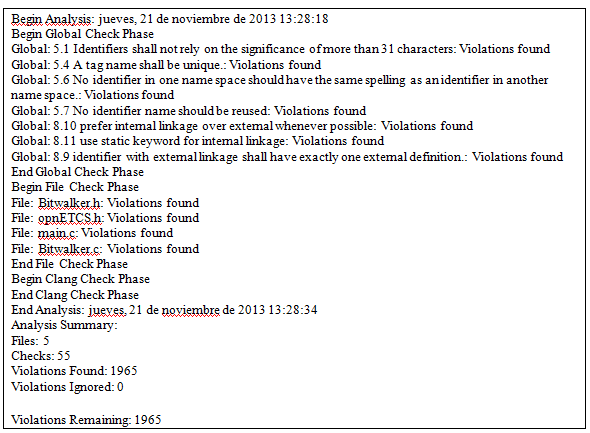
\includegraphics{./figures/understand.png}
\caption{MISRA-C Rules results}
\end{figure}

The files into the violations are found are listed in the below table.

{\footnotesize\sffamily\centering
  \begin{longtable}{||p{.15\textwidth}|p{.8\textwidth}||}
  \caption{Ubication of MISRA Violations}\\
    \hline\hline
    \textbf{MISRA Rule} & \textbf{Files} \\
    \hline\hline
    \endhead
    \hline\hline
    \endfoot
    \textbf{Global 5.1}
& Bitwalker.c/opnETCS.h/opnETCS\_Decoder.h
    \\
    \hline
    \textbf{Global 5.4}
& opnETCS.h
    \\
    \hline
    \textbf{Global 5.6}
& Bitwalker.c/Bitwalker.h
    \\
    \hline
    \textbf{Global 5.7}
& Bitwalker.c/Bitwalker.h/opnETCS.h
    \\
    \hline
    \textbf{Global 8.9}
& opnETCS\_Decoder.h
    \\
    \hline
    \textbf{Global 8.10}
& main.c
    \\
    \hline
    \textbf{Global 8.11}
& main.c
    \\
    \hline
\end{longtable}}

\subsection{Clang Static Analyzer tool Results}
The Clang Static Analyzer is a source code analysis tool that finds bugs in C, C++, and Objective-C programs.

The analyzer is 100\% open source and is part of the Clang project. Like the rest of Clang, the analyzer is implemented as a C++ library that can be used by other tools and applications.

With this analysis SQS has checked the following:

{\footnotesize\sffamily\centering
  \begin{longtable}{||p{.45\textwidth}|p{.5\textwidth}||}
  \caption{Aspects checked}\\
    \hline\hline
    \hline\hline
    \endhead
    \hline\hline
    \endfoot
    \textbf{core.AdjustedReturnValue}
& Check to see if the return value of a function call is different than the caller expects (e.g., from calls through function pointers).
    \\
    \hline
    \textbf{core.CallAndMessage}
& Check for logical errors for function calls and Objective-C message expressions (e.g., uninitialized arguments, null function pointers).
    \\
    \hline
    \textbf{core.DivideZero}
& Check for division by zero.
    \\
    \hline
    \textbf{core.NonNullParamChecker}
& Check for null pointers passed as arguments to a function whose arguments are known to be non-null.
    \\
    \hline
    \textbf{core.NullDereference}
& Check for dereferences of null pointers.
    \\
    \hline
    \textbf{core.StackAddressEscape}
& Check that addresses to stack memory do not escape the function.
    \\
    \hline
    \textbf{core.UndefinedBinaryOperatorResult}
& Check for undefined results of binary operators.
    \\
    \hline
    \textbf{core.VLASize}
& Check for declarations of VLA of undefined or zero size.
    \\
    \hline
    \textbf{core.builtin.BuiltinFunctions}
& Evaluate compiler built-in functions (e.g., alloca()).
    \\
    \hline
    \textbf{core.builtin.NoReturnFunctions}
& Evaluate "panic" functions that are known to not return to the caller.
    \\
    \hline
    \textbf{core.uninitialized.ArraySubscript}
& Check for uninitialized values used as array subscripts.
    \\
    \hline
    \textbf{core.uninitialized.Assign}
& Check for assigning uninitialized values.
    \\
    \hline
    \textbf{core.uninitialized.Branch}
& Check for uninitialized values used as branch conditions.
    \\
    \hline
    \textbf{core.uninitialized.CapturedBlockVariable}
& Check for blocks that capture uninitialized values.
    \\
    \hline
    \textbf{core.uninitialized.UndefReturn}
& Check for uninitialized values being returned to the caller.
    \\
    \hline
    \textbf{cplusplus.NewDelete}
& Check for double-free and use-after-free problems involving C++ delete.
    \\
    \hline
    \textbf{deadcode.DeadStores}
& Check for values stored to variables that are never read afterwards.
    \\
    \hline
    \textbf{osx.API}
& Check for proper uses of various Apple APIs.
    \\
    \hline
    \textbf{osx.SecKeychainAPI}
& Check for proper uses of Secure Keychain APIs.
    \\
    \hline
    \textbf{osx.cocoa.AtSync}
& Check for nil pointers used as mutexes for @synchronized.
    \\
    \hline
    \textbf{osx.cocoa.ClassRelease}
& Check for sending 'retain', 'release', or 'autorelease' directly to a Class.
    \\
    \hline
    \textbf{osx.cocoa.IncompatibleMethodTypes}
& Warn about Objective-C method signatures with type incompatibilities.
    \\
    \hline
    \textbf{osx.cocoa.NSAutoreleasePool}
& Warn for suboptimal uses of NSAutoreleasePool in Objective-C GC mode.
    \\
    \hline
    \textbf{osx.cocoa.NSError}
& Check usage of NSError** parameters.
    \\
    \hline
    \textbf{osx.cocoa.NilArg}
& Check for prohibited nil arguments to ObjC method calls.
    \\
    \hline
    \textbf{osx.cocoa.RetainCount}
& Check for leaks and improper reference count management.
    \\
    \hline
    \textbf{osx.cocoa.SelfInit}
& Check that 'self' is properly initialized inside an initializer method.
    \\
    \hline
    \textbf{osx.cocoa.UnusedIvars}
& Warn about private ivars that are never used.
    \\
    \hline
    \textbf{osx.cocoa.VariadicMethodTypes}
& Check for passing non-Objective-C types to variadic methods that expect only Objective-C types.
    \\
    \hline
    \textbf{osx.coreFoundation.CFError}
& Check usage of CFErrorRef* parameters.
    \\
    \hline
    \textbf{osx.coreFoundation.CFNumber}
& Check for proper uses of CFNumberCreate.
    \\
    \hline
    \textbf{osx.coreFoundation.CFRetainRelease}
& Check for null arguments to CFRetain/CFRelease/CFMakeCollectable.
    \\
    \hline
    \textbf{osx.coreFoundation.containers.OutOfBounds}
& Checks for index out-of-bounds when using 'CFArray' API.
    \\
    \hline
    \textbf{osx.coreFoundation.containers.PointerSizedValues}
& Warns if 'CFArray', 'CFDictionary', 'CFSet' are created with non-pointer-size values.
    \\
    \hline
    \textbf{security.FloatLoopCounter}
& Warn on using a floating point value as a loop counter (CERT: FLP30-C, FLP30-CPP).
    \\
    \hline
    \textbf{security.insecureAPI.UncheckedReturn}
& Warn on uses of functions whose return values must be always checked.
    \\
    \hline
    \textbf{security.insecureAPI.getpw}
& Warn on uses of the 'getpw' function.
    \\
    \hline
    \textbf{security.insecureAPI.gets}
& Warn on uses of the 'gets' function.
    \\
    \hline
    \textbf{security.insecureAPI.mkstemp}
& Warn when 'mkstemp' is passed fewer than 6 X's in the format string.
    \\
    \hline
    \textbf{security.insecureAPI.mktemp}
& Warn on uses of the 'mktemp' function.
    \\
    \hline
    \textbf{security.insecureAPI.rand}
& Warn on uses of the 'rand', 'random', and related functions.
    \\
    \hline
    \textbf{security.insecureAPI.strcpy}
& Warn on uses of the 'strcpy' and 'strcat' functions.
    \\
    \hline
    \textbf{security.insecureAPI.vfork}
& Warn on uses of the 'vfork' function.
    \\
    \hline
    \textbf{unix.API}
& Check calls to various UNIX/Posix functions.
    \\
    \hline
    \textbf{unix.Malloc}
& Check for memory leaks, double free, and use-after-free problems involving malloc.
    \\
    \hline
    \textbf{unix.MallocSizeof}
& Check for dubious malloc arguments involving sizeof.
    \\
    \hline
    \textbf{unix.MismatchedDeallocator}
& Check for mismatched deallocators (e.g. passing a pointer allocating with new to free()).
    \\
    \hline
    \textbf{unix.cstring.BadSizeArg}
& Check the size argument passed into C string functions for common erroneous patterns.
    \\
    \hline
    \textbf{unix.cstring.NullArg}
& Check for null pointers being passed as arguments to C string functions.
    \\
    \hline
\end{longtable}}

After run this analysis no violations have been found.

\begin{figure}[H]
\centering
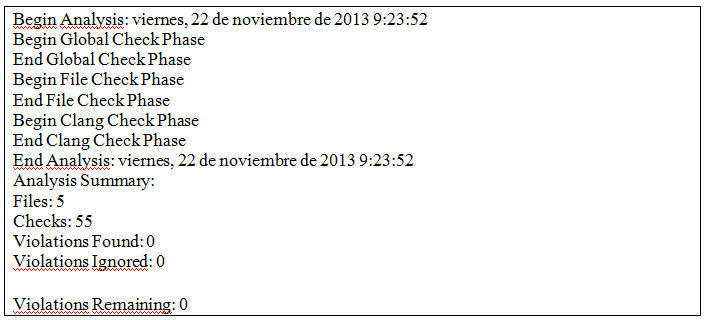
\includegraphics[scale=0.8]{./figures/clang.png}
\caption{Clang Analysis results}
\end{figure}

\subsection{CPPcheck tool Results}

Bitwalker folder has been analyzed statically by CPPcheck tool (Complying with the standard C11).
 C11 (formerly C1X) is an informal name for ISO/IEC 9899:2011, the current standard for the C programming language. It replaces the previous C standard, informally known as C99. This new version mainly standardizes features that have already been supported by common contemporary compilers, and includes a detailed memory model to better support multiple threads of execution. Due to delayed availability of conforming C99 implementations, C11 makes certain features optional, to make it easier to comply with the core language standard.
 
The results of the tool are the following:
\begin{figure}[H]
\centering
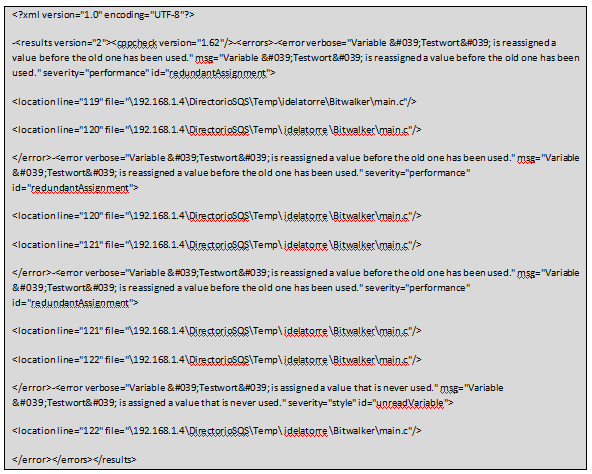
\includegraphics{./figures/cppcheck.png}
\caption{cppcheck results}
\end{figure}

\subsection{Results Comparison}
\cleardoublepage
%
\chapter{Conclusions}
\label{sec:conclusions}

\fxfatal{issue 169: As the bitwalker example allows a limited usage of the approach, could you give in conclusion some feedbacks from previous experience ? in which case this approach is efficient to be used ?}

\fxfatal{issue 169: This report presents experiment swith two complementary approaches, is it possible to have in conclusion some comments on which approach is recommended to be used in the openETCS project, on which artifacts and to cover which objectives of VnV ? Then which steps of VnV are expected to cover EN50128 requirements and are not covered by these approaches ?}
\cleardoublepage


\bibliographystyle{unsrt}
\bibliography{bibliography}

\nocite{*}
%===================================================
%Do NOT change anything below this line

\end{document}
